\chapter{Design and Implementation of Wireguard for GNRC}
This chapter covers the specific requirements for the Wireguard adaptation for GNRC, the design 
details to meet the requirements and important implementation aspects inside the Wireguard source
code for RIOT.
\section{Requirements}
  \begin{itemize}
    \item \textbf{Static memory allocation}: Dynamic memory allocation is prohibited within RIOT core 
    components to maintain a predictable runtime memory usage and real-time performance. With
    Wireguard being at the layer 3 of the network stack, the protocol must use static memory
    allocation exclusively.
    \item \textbf{Security}: The GNRC implementation needs to be align to the security properties that
    the original Linux implementation holds. This includes the resistant to replay attack and
    side-channel attack \cite{side}, perfect forward secrecy, low probability of handshake collision \cite{pwu}
    ,cryptographic soundness, and safety from concurrency bugs.
    \item \textbf{Interconnectiviy with other Wireguard implementation}: The RIOT adaptation must 
    be able to communicate with other RIOT Wireguard node and obviously the Linux implementation.
    \item \textbf{Integration to RIOT network interfaces API}: Similiar to the Linux implementation,
    Wireguard will be an network interface, receive IPv6 packets from the layer above, and
    hande the all the encryption and dispatching.
    \item \textbf{6LoWPAN compatiblility}: The Wireguard implementation only supports IPv6 packet
    to be compatible with the 6LoWPAN layer.
  \end{itemize}
\section{Event-driven architecture}
  Taking inspiration from BoringTun \cite{boringtun}, the Wireguard implementation handles
  packets and timers in an event-oriented manner. Three different kinds of event can occur within
  a Wireguard session:
  \begin{itemize}
    \item Transmitting data from the IP layer.
    \item Reception of a packet from any peer.
    \item The timeout event related to the Wireguard timers.
  \end{itemize}

  \begin{figure}[h]
    \centering
    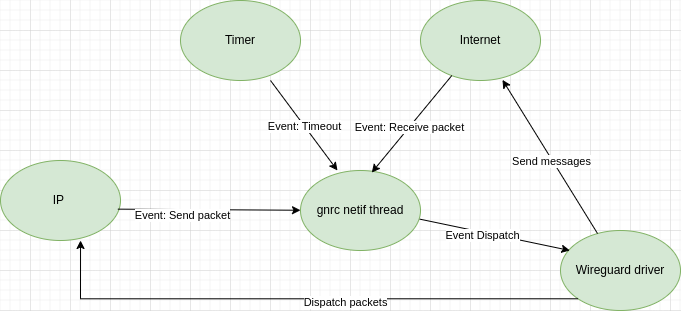
\includegraphics[width=\linewidth]{wireguard}
    \caption{GNRC Wireguard Software Architecture}
    \label{fig:wireguard}
  \end{figure}

  Figure \ref{fig:wireguard} illustrates the overview of the architecture of the GNRC Wireguard
  implementation. The Wireguard driver is the core component where it executes the Noise handshake,
  handles the functions triggered by the timeout event, encrypts, decrypts and transmits packet to
  the IP layer or the internet outside. To make use of the existing RIOT system, the GNRC netif's
  event queue is used as the central event listener for all 3 types of event. 
  
  Whenever, a packet is received on the UDP port of Wireguard, new event to handle the reception will be pushed
  at the netif's event queue, letting Wireguard make the decision whether to responde to 
  the peer if the packet is a handshake message, dispatch the packet directly to the IP layer if 
  it is authenticated or discard if the packet is invalid. 

  An IP layer will mostly be unaware of the inner working of Wireguard, as it will only transmit the
  packet to the specified netif and receives the pre-processed IPv6 packet from the driver. One thing
  to note is that the Linux implementation of Wireguard will queue the packets for another thread
  to process. The GNRC also follows that design, but with smaller packet queue to match the
  constrained environment.

  Every expiration of a timer, like timer for retransmission of the handshake or passing the
  keepalive, the event will also be pushed on top of the event queue for the driver to handle later.
  
  The design reduces the complexity of concurrency, as every event is handled sequentially, making it impossible for 
  other threads to
  meddle with the inner cryptography state of the driver. Although it could make the netif thread
  a bottleneck of performance, the thread would not be overload in a normal circumstance of
  IoT environment.

\section{Network Interfaces API}
  Show the supported API.

  create a netif thread like any other netif.
  
  Mention on the connect problem to start the handshake initation first. Disconnect will
  disconnect from a peer only. 

  Shutdown will clean all the peer state of Wireguard. 
  
  The netif peer contains the configuration of the peer on the Wireguard drivers.

  Init the peer with default configuration. Adding the peer is concurrently safe as with a 
  central lock around the list of peer. Allow
  to add the IPv6 address on a netif like a a normal netif would do.
\section{Memory allocation \& optmization}
  The number of peers must be preconfigured, hence the memory for peers are statically configured
  before hand. Peer that are freed marks with a boolean variable valid to known
  the peer is usable by other thread or not.

  Every search for keypair, generation of index or look up based on the index, allowed ip
  are linear iteration over all the peer.

  Instread of Making Wireguard running in its own thread, running in its own event loop
  with its own queue, Wireguard drivers run in the same thead as the netif, making 
  use of the existing netif event queue structure and msg box of netif to the handle.
  Although it enforces an order, however as the sending of packet should know beforehand
  to ensure the realtime cap, the packet queue won't be overload with the number of concurrent
  events.

  There is a packet queue, but only allows the total maximum of the number of peer multiplied by 2.
  This comes from the assumption is the device either send packet periodically, or sometimes
  do the sending. If the packet queue is full and there in no handshake session, the packet 
  is simply discarded.

  To reduce the fragmentation, the realloation and the merging of data happens only one during the final preparation
  of the transport message. The code is a follow, first we allocate enough space for the padded
  packet and the header. Then copy all the payload after the IPv6 to the end, then slide
  the orignal IPv6 header to its right place.

\section{Security Requirements \& Implementations}
  The packet is silently drop if it no valid. crypto{\_}secure{\_}wipe and crypto{\_}equals are used to
  handle the comparsion between the keypairs, and the wipe out of the packet state. ensuring
  there is no leaking.
  
  The ECDH implementation include an additional check for zero bytes to prevent the zero public 
  key.

  Less likey to have concurency bugs because of the sequential nature to handle all the noise 
  handshake. 

  Crypto primitve is implemented in the same way as the Linux does.

  Regarding the under load condition to prevent the DoS, seemly counter the number of event on the
  event queue, as it thread allow to hanle 16 events at once, the limitation of the number of
  event is 16 before handle the final handshake, instead sending out the cookie is 12 events at a time.
\section{Implementation Status}
  Finished features:
    handling of Noise handshake state 
    support of every wireguard messages.
    timer state machine
    packet queuing.

  functional enough to communicate with the Linux implementation.
  
  Missing features:
    private key configuration
    removal of peers

  Problems:
     on the neighbor cache entry to dispatcht the packet out, still required to install
     the entry to support sending to the endpoint. 